\documentclass[letterpaper,fleqn]{article}
\usepackage[spanish,es-noshorthands]{babel}
\usepackage[utf8]{inputenc} 
\usepackage[left=1cm, right=1cm, top=1.5cm, bottom=1.7cm]{geometry}
\usepackage{mathexam}
\usepackage{amsmath,amsthm,amsfonts,amssymb}
\usepackage{graphicx}
\usepackage{tikz,pgf}
\usepackage{multicol}

\ExamClass{
\includegraphics[height=16pt]{Images/logo-sed.png} Matemáticas $11^{\circ}$}
\ExamName{Nivelación Período 1}
\ExamHead{
\includegraphics[height=16pt]{Images/logo-colegio.png} IEDAB}
\newcommand{\LineaNombre}{%
\par
\vspace{\baselineskip}
Nombre:\hrulefill \; Curso: \underline{\hspace*{48pt}} \; Fecha: \underline{\hspace*{2.5cm}} \relax
\par}
\let\ds\displaystyle

\begin{document}
\ExamInstrBox{
Respuesta sin justificar mediante procedimiento no será tenida en cuenta en la calificación. Escriba sus respuestas en el espacio indicado. Tiene 45 minutos para contestar esta prueba.}
\LineaNombre
\begin{enumerate}
   \item Sobre la línea, determine la propiedad de los números reales que se ha usado:
  \begin{enumerate}
    \item $ (x+y)(v-w)=(v-w)(x+y) $ \underline{\hspace{6cm}}
    \item $ (A+B)(x+y)=(A+B)x+(A+B)y $ \underline{\hspace{6cm}}
  \end{enumerate}
  \item Exprese cada intervalo como una desigualdad y luego grafíquela en la recta dispuesta para ello.
  
  \begin{enumerate}
    \item $ [-2,4) $ \underline{\hspace{6cm}}
    \vspace{20pt}
    \begin{flushright}
    \begin{tikzpicture}[scale=.8,>=stealth]
\draw[<->] (0,0) -- (12,0);
\draw [thick] (1,-.1) -- (1,0.1);
\draw [thick] (2,-.1) -- (2,0.1);
\draw [thick] (3,-.1) -- (3,0.1);
\draw [thick] (4,-.1) -- (4,0.1);
\draw [thick] (5,-.1) -- (5,0.1);
\draw [thick] (6,-.1) -- (6,0.1);
\draw [thick] (7,-.1) -- (7,0.1);
\draw [thick] (8,-.1) -- (8,0.1);
\draw [thick] (9,-.1) -- (9,0.1);
\draw [thick] (10,-.1) -- (10,0.1);
\draw [thick] (11,-.1) -- (11,0.1);
\end{tikzpicture}
    \end{flushright}\vspace{20pt}

  \end{enumerate}
  \item Exprese en notación de intervalos y luego grafique el correspondiente intervalo:
  \begin{enumerate}
    \item $ x\leq 2 $ \noanswer
     \begin{flushright}
  \begin{tikzpicture}[scale=.8,>=stealth]
\draw[<->] (0,0) -- (12,0);
\draw [thick] (1,-.1) -- (1,0.1);
\draw [thick] (2,-.1) -- (2,0.1);
\draw [thick] (3,-.1) -- (3,0.1);
\draw [thick] (4,-.1) -- (4,0.1);
\draw [thick] (5,-.1) -- (5,0.1);
\draw [thick] (6,-.1) -- (6,0.1);
\draw [thick] (7,-.1) -- (7,0.1);
\draw [thick] (8,-.1) -- (8,0.1);
\draw [thick] (9,-.1) -- (9,0.1);
\draw [thick] (10,-.1) -- (10,0.1);
\draw [thick] (11,-.1) -- (11,0.1);
\end{tikzpicture}
  \end{flushright}
  \end{enumerate}
  \item Realice las operaciones indicadas, simplificando siempre que sea posible:
  \begin{enumerate}
    \item $ 5+\frac{3}{5}-\frac{1}{4}= $ \vspace{45pt}
    \item $ 0.25(\frac{5}{7}+\frac{2}{5})= $ \vspace{45pt}
    \item $ (\frac{3}{4}-\frac{2}{5})(\frac{1}{6}-\frac{1}{4})= $ \vspace{45pt}
    \item $ \dfrac{5-\frac{2}{5}}{\frac{1}{4}-\frac{1}{3}}= $ \vspace{45pt}
  \end{enumerate}
  \item Ubique el símbolo correcto ($<$ ,$>$, o $=$) en el espacio:
  \begin{enumerate}\begin{multicols}{2}
    \item $ 6 $ \underline{\hspace{.7cm}} $ \frac{19}{3} $
    \item $ \frac{2}{3} $ \underline{\hspace{.7cm}} $ 0.66 $
    \item $ -4 $ \underline{\hspace{.7cm}} $ -\frac{17}{4} $
    \item $ |-0.95| $ \underline{\hspace{.7cm}} $ |0.95| $
    \end{multicols}
  \end{enumerate}
  \item Exprese como una desigualdad las siguientes expresiones:
  \begin{enumerate}
    \item $ q $ es menor que 6 y mayor o igual que $ -3 $ \hspace*{1cm} \underline{\hspace*{4cm}}
    \item $3x$ es positivo \hspace*{1cm} \underline{\hspace*{4cm}}
  \end{enumerate}
  \item Al lanzar dos dados, calcular la probabilidad
  \begin{enumerate}
  \item Que su suma sea que 8
  \item Que su suma sea menor o igual que 5
  \end{enumerate}
   \section*{Preparándonos para la Prueba Saber}
\item Se desea adquirir un terreno de forma cuadrada con un perímetro entre 4 y 20 metros. Si $x$ representa el lado del terreno, los valores que puede tomar $x$ para que el
perímetro del terreno cumpla la condición dada son
\begin{enumerate}
\begin{multicols}{4}
\item $4<x<20$
\item $0<x<16$
\item $2<x<10$
\item $1<x<5$
\end{multicols}
\end{enumerate}
\begin{minipage}{.4\textwidth}
\item Andrea construyó una cometa con cuatro triángulos de papel que cortó de dos rectángulos con las medidas que se señalan en los dibujos
\end{minipage}
\begin{minipage}{.55\textwidth}
\begin{tikzpicture}[scale=.95]
\draw (0,0) rectangle (4,3);
\node  at (1,2.5) {Triangulo 1};
\draw[dashed] (0,0) --node {50cm} (4,3);
\node  at (2.75,.5) {Triangulo 2};
\draw[|-|](0,-.2)--node[below]{40cm}(4,-.2);
\draw[|-|] (4.2,0)--node[right]{30 cm}(4.2,3); 
\draw (6,0) rectangle (8,1.5);
\draw[dashed] (6,0)--node{25cm}(8,1.5);
\node at (6.7,1.2){Triang 3};
\node at (7.2,.2){Triang 4};
\draw[|-|] (8.2,0)--node[right]{15 cm}(8.2,1.5);
\end{tikzpicture} 
\end{minipage}

\begin{minipage}{.5\textwidth}
\begin{tikzpicture}[scale=.9]
\draw (0,0) -- (6,0) --(3,4)node[above]{$K$}--cycle;
\draw (3,4)--(3,-2);
\draw (1.5,0)--(3,-2)node[below]{$S$}--(4.5,0);
\draw[dashed,|-|](3.1,4.1)--node[right]{50 cm}(6.1,0.1);
\node (1) at (1.35,.65) {Triangulo 1};
\node (2) at (4.35,.7) {Triangulo 2};
\node (3) at (2.2,-.2) {Triang 3};
\node (4) at (3.7,-.2) {Triang 4};
\draw[dashed,|-|](3,.15)--node[above]{15cm}(4.5,.15);
\end{tikzpicture}
\end{minipage}
\begin{minipage}{.45\textwidth}
La cometa armada tiene la forma anterior:
\end{minipage}
La distancia entre los puntos $K$ y $S$ es
\begin{enumerate}
\begin{multicols}{4}
\item 40 cm
\item 55 cm
\item 60 cm
\item 75 cm
\end{multicols}
\end{enumerate}

    \begin{minipage}{.4\textwidth}
      \item Si se lanza un caja de fósforos, ésta puede caer en cualquiera de las posiciones de la figura.
  \end{minipage}\hfill
  \begin{minipage}{.55\textwidth}
    \begin{center}
  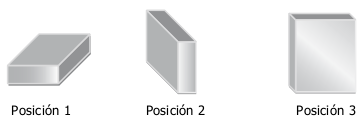
\includegraphics[scale=.55]{Images/fosforos.png}
  \end{center}
  \end{minipage}
  \begin{minipage}{.5\textwidth}
      \begin{center}
  \begin{tabular}{|c|c|}\hline
  \textbf{Posición}&\textbf{Probabilidad estimada}\\\hline
    1 & $ p(1)=0,65 $\\\hline
    2 & $ p(2)=0,22 $\\\hline
    3 & $ p(3)=0,13 $\\\hline
  \end{tabular}
  \end{center}
  \end{minipage}\hfill
  \begin{minipage}{.45\textwidth}
    La tabla construída después de efectuar 100 lanzamientos, muestra la probabilidad de caída en cada posición.
  \end{minipage}
  
  Después de otros cien lanzamientos más, se espera que
  \begin{enumerate}
    \item más de la mitad de las posiciones de caída corresponda a las posiciones 2 y 3
    \item las tres posiciones tengan aproximadamente la misma probabilidad entre ellas
    \item más de la mitad de todas las posiciones de caída corresponda a la posición 1
    \item el número de veces que cae la caja en la posición 2 se aproxime al 50\%
  \end{enumerate}
\end{enumerate}
\end{document}
